\documentclass[9pt]{beamer}
\usepackage{styles/mypreamble}
%~~~~~~~~~~~~~~~~~~~~~~~~~~~~~~~~~~~~~~~~~~~~~~~~~~~~~~~~~~~~~~~~~~~~~~~~~~~~~~
\title{Алгоритмы машинного обучения}
\subtitle{Лекция 1. Что такое машинное обучение. Обзор курса.}
\author{Владимир Кукушкин}
\institute{СПбГЭУ - 11.11.2020}
%~~~~~~~~~~~~~~~~~~~~~~~~~~~~~~~~~~~~~~~~~~~~~~~~~~~~~~~~~~~~~~~~~~~~~~~~~~~~~~

\begin{document}
\titlepage

\section{Мотивация}

\subsection{N причин заниматься анализом данных}

\begin{frame}{Это интересно}
    \begin{itemize}
        \item Данные -- нефть 21го века.
        \item Data science находится на стыке статистики, теории вероятности и computer science.
        \item Это настоящий современный rocket science. Некоторые методы, которые будем рассматривать в курсе, появились на свет только в 2018 году. По многим методам ещё не написаны книги: единственными источниками информации являются статьи-первоисточники, и обсуждения на тематических ресурсах.
        \item Часто приходится прибегать к методам "чёрной магии"\;-- эвристикам, которые подходят исключительно к вашей задаче/данным.
        \item Существует множество конкурсов, в которых можно начинающим отточить навыки, а профессионалам ещё и заработать. И это азартно. См. \url{https://kaggle.com}.
    \end{itemize}
\end{frame}

\begin{frame}{Это востребовано}
\begin{center}
    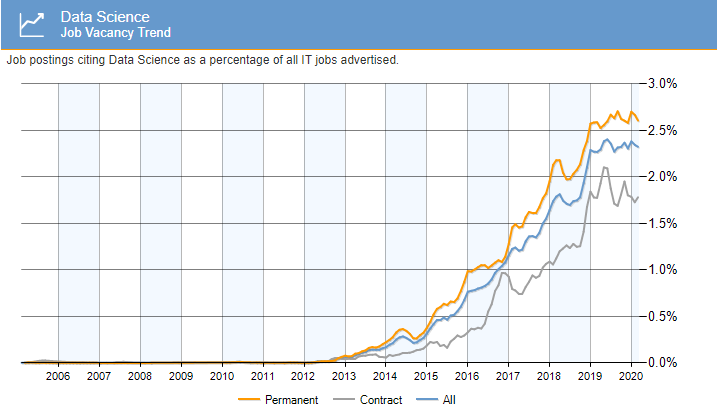
\includegraphics[width=0.9\textwidth]{img/intro_job_trend.png}
\end{center}
\url{https://www.icertglobal.com/what-will-be-the-job-scenario-for-data-science-in-2020/detail}
\end{frame}

\begin{frame}{Это прибыльно}
\begin{center}
    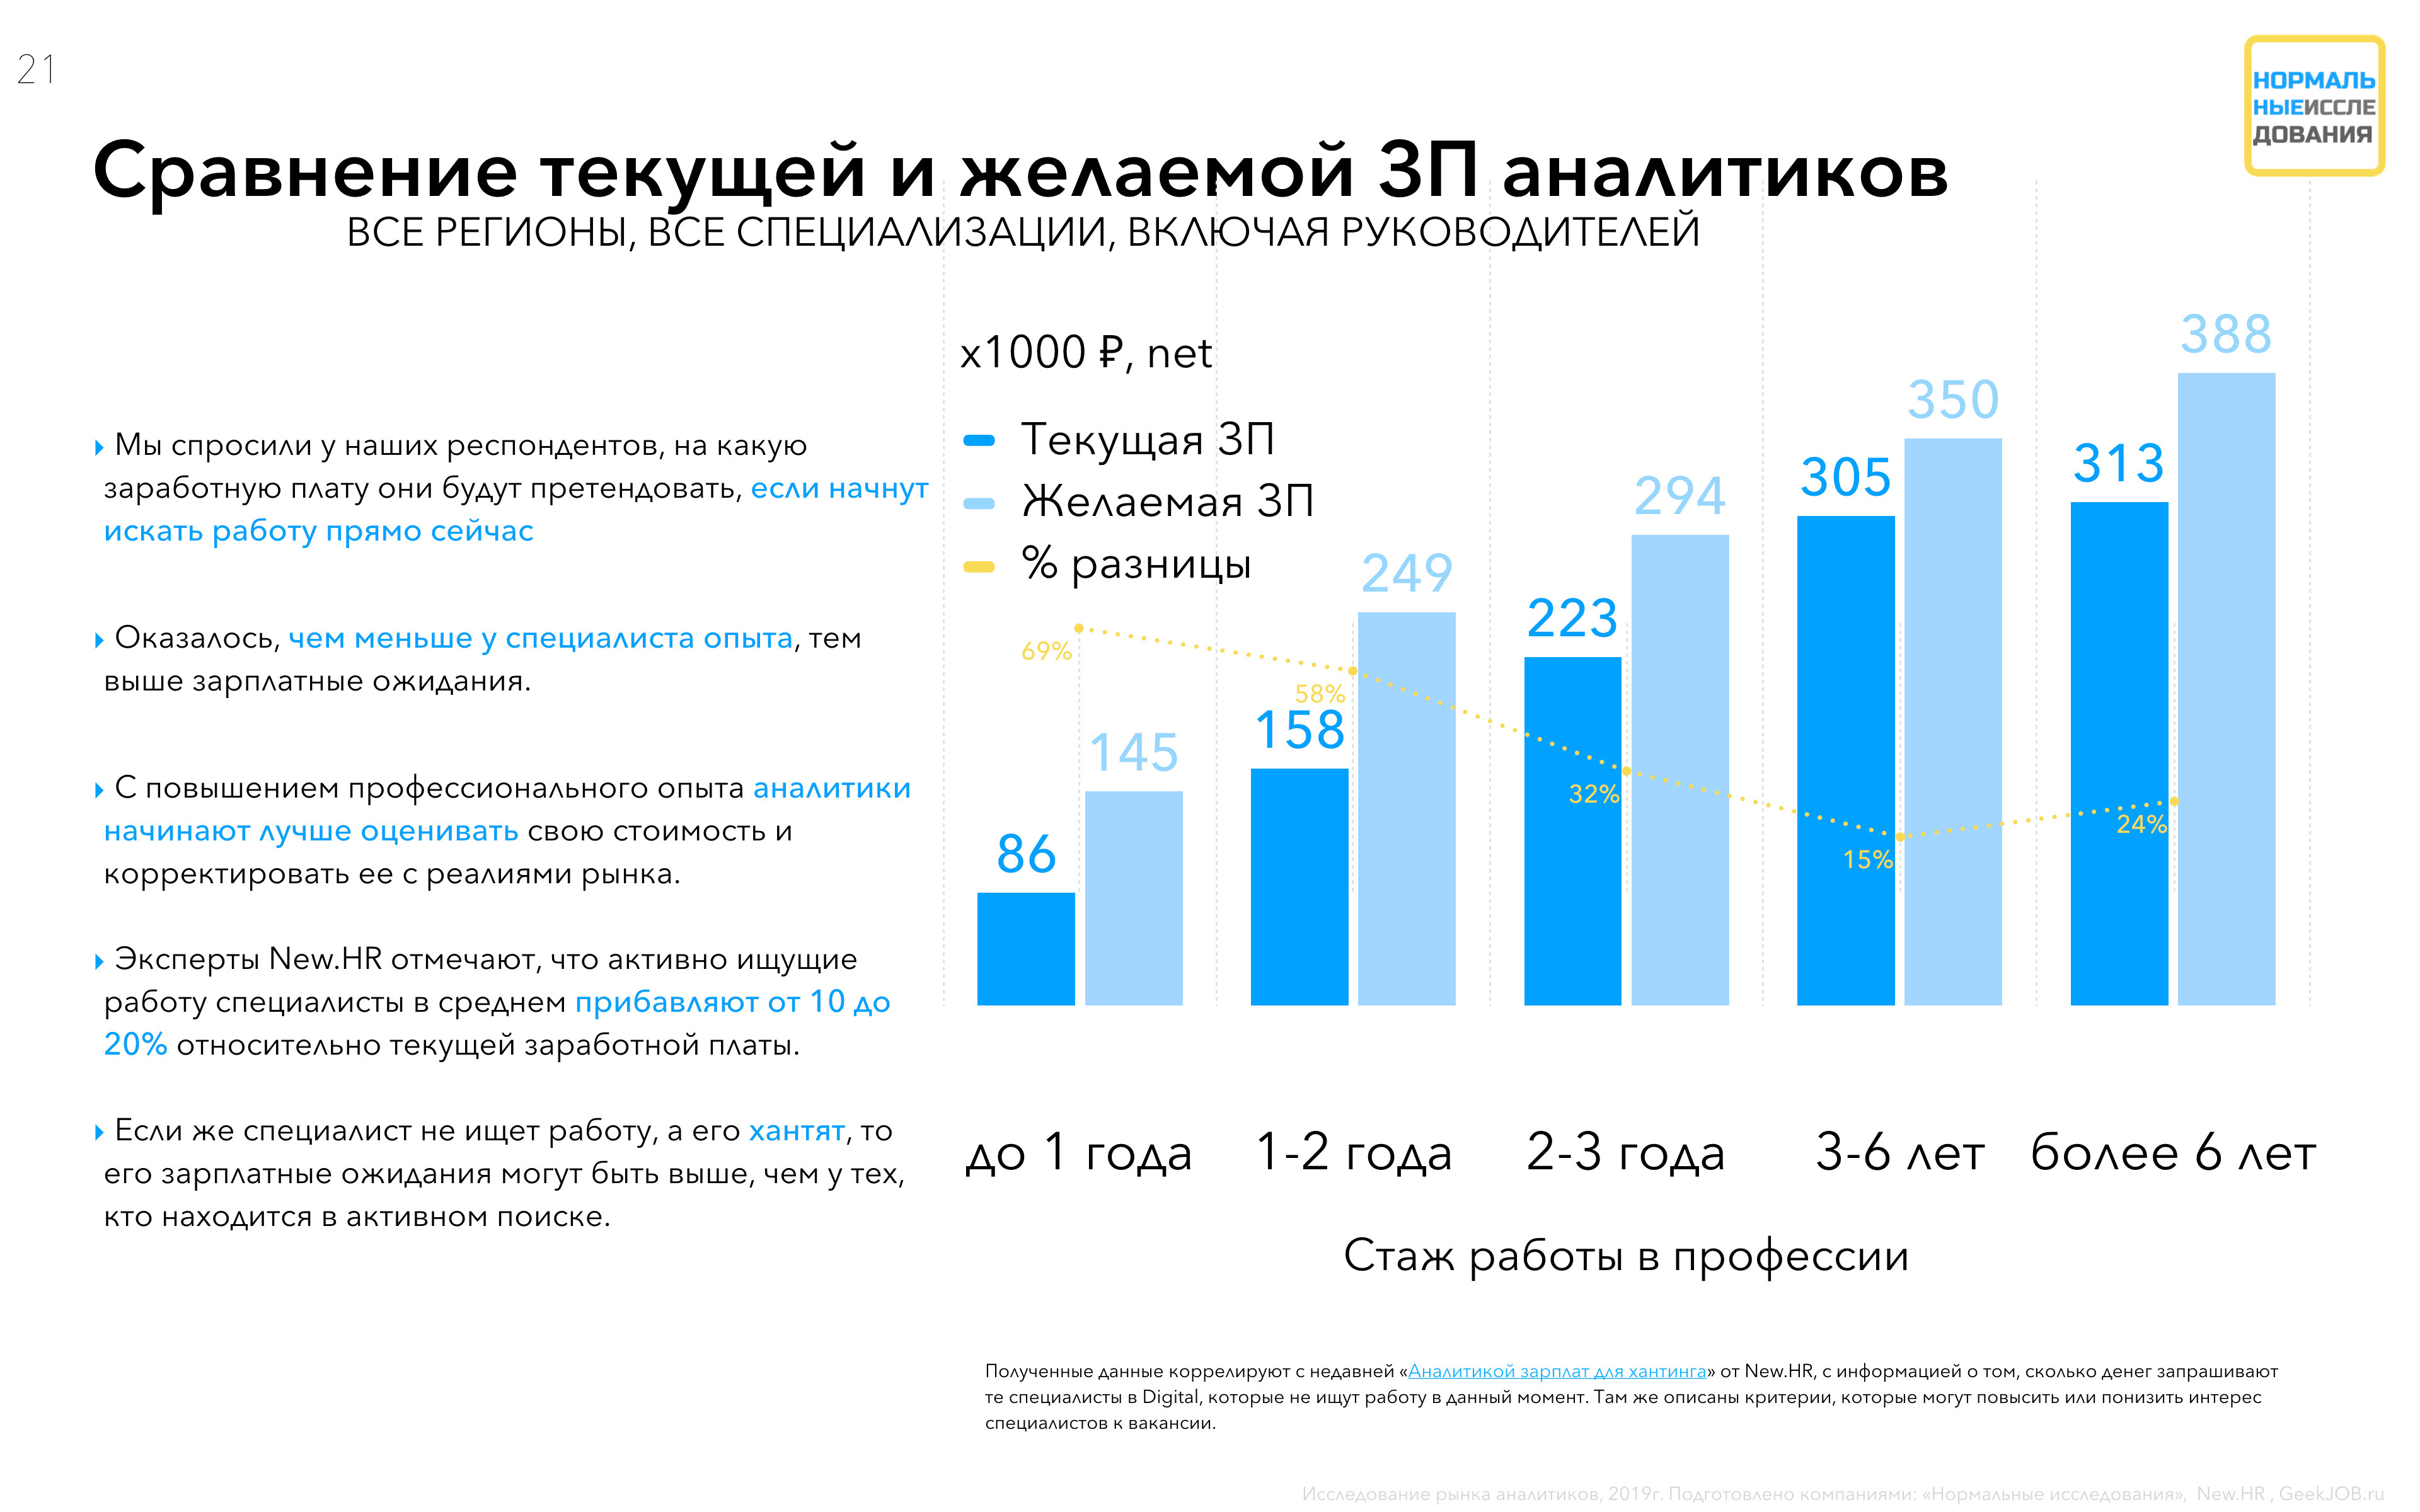
\includegraphics[width=0.9\textwidth]{img/intro_data_scientist_wage.png}
\end{center}
\url{https://vc.ru/hr/82631-issledovanie-rynka-analitikov}
\end{frame}

\begin{frame}{Это прибыльно}
\begin{center}
    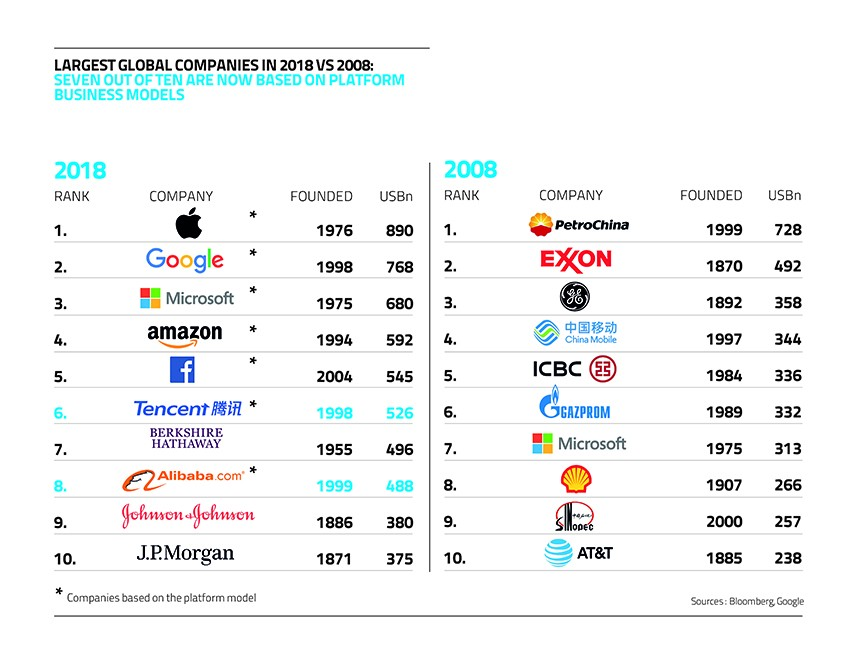
\includegraphics[width=0.8\textwidth]{img/intro_it_companies.jpeg}
\end{center}
\url{https://innovator.news/the-platform-economy-3c09439b56}
\end{frame}

\begin{frame}{Почему так?}
    \begin{itemize}
        \item Вариант закон Мура для данных: \href{https://medium.com/alectio/why-the-end-of-moores-law-means-the-end-of-big-data-as-we-know-it-7e77477c70a0}{90\% всех имеющихся данных сгенерировано было сгенерировано с 2016 года} (к 2019 году на момент написания статьи).
        \item \href{https://solutionsreview.com/data-management/80-percent-of-your-data-will-be-unstructured-in-five-years/}{80\% из этих данных неструктурированы}.
        \item И всё это добро надо как-то анализировать.
    \end{itemize}
\end{frame}

\begin{frame}{Почему так?}
\begin{center}
    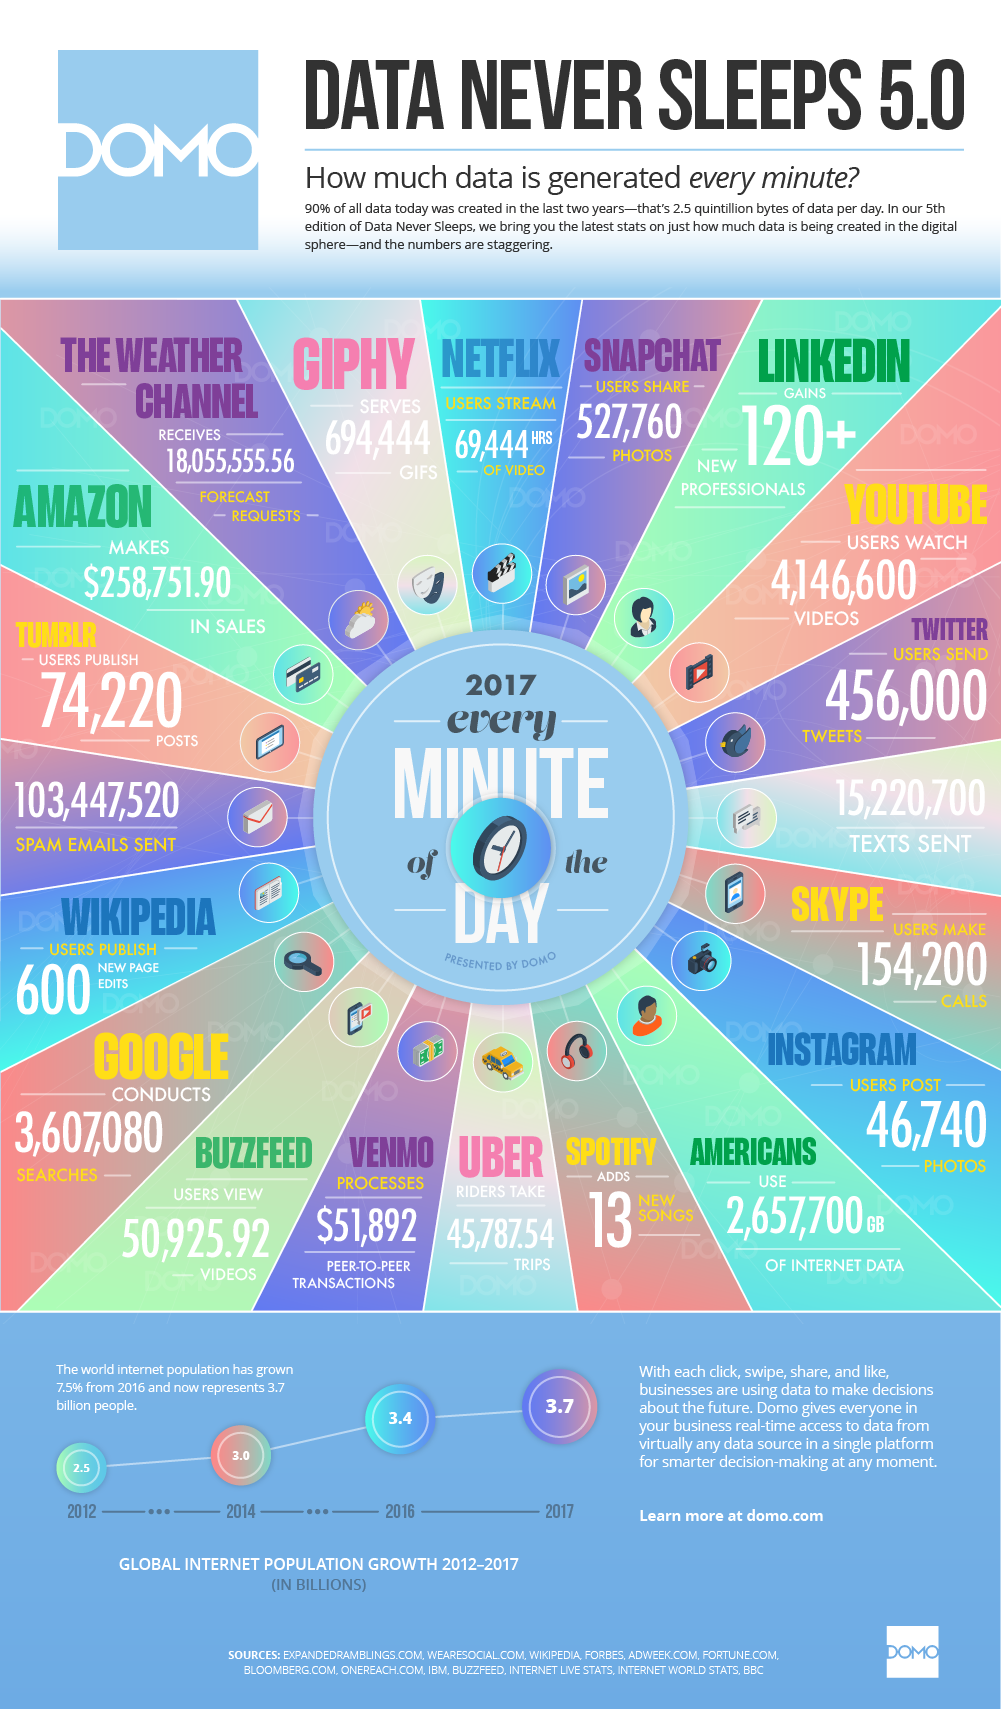
\includegraphics[height=0.7\textheight]{img/intro_data_every_minute.png}
\end{center}
\url{https://www.domo.com/learn/data-never-sleeps-5?aid=ogsm072517_1&sf100871281=1}
\end{frame}

\subsection{Чем занимаются data analyst и data scientist}
\begin{frame}{Что изучает data analyst}
Грубо говоря, аналитик -- это тот, кто выполняет анализ данных, не связанный с машинным обучением. А именно:
\begin{itemize}
    \item Построение систем метрик и дашбордов.
    \item Поверхностный анализ пользовательского поведения. Конверсии, воронки, CJM (Customer Journey Map), отток и привлечение пользователей.
    \item Финансовые расчёты: выручка, прогнозирование выручки, юнит-экономика.
    \item Принятие бизнес-решений. AB-тестирование. Генерация идей, проверка статистических гипотез, проведение экспериментов.
    \item Data-engineering задачи: преобразование данных из сырых логов в удобовариваемый вид (для использования и хранения), построение пайплайнов для обработки данных, проверка консистентности данных, определение разладок.
\end{itemize}
\end{frame}

\begin{frame}{Главные инструменты аналитика}
    \begin{itemize}
        \item Для получения данных: SQL, Hadoop+Hive, Clickhouse.
        \item Общие языки программирования: Python (в особенности pandas), R. Для инженерных задач ещё и bash.
        \item Средства визуализации: Tableau, Power BI, Periscope.
        \item Для аналитики событий: Яндекс.Метрика, Google.Analytics.
    \end{itemize}
\end{frame}

\begin{frame}{Что изучает data scientist}
Дата саентист больше про машинное обучение (artificial intelligence, если хотите), алгоритмы, математику и программирование. Типичные задачи:
\begin{itemize}
    \item Настроить классификатор, предсказывающий что угодно (события покупки, возврата кредита, выручку, загрузку приложения).
    \item Доказать, что новая модель действительно лучше предыдущей.
    \item Внедрить настроенную модель. Добиться того, чтобы модель эффективно работала в продакшене (достаточно быстро, не требовала терабайтов данных, можно было разобраться в принятии решений и т.д.).
    \item Глубокий анализ пользовательского поведения.
\end{itemize}
Главные инструменты:
\begin{itemize}
    \item Для получения данных: SQL, Hadoop+Hive, Clickhouse.
    \item Общие языки программирования: Python (в особенности scikit-learn), R. Для инженерных задач ещё и bash. В некоторых случаях Spark, Julia.
    \item Jupyter и PyCharm как среда разработки.
    \item (Python-)фреймворки для нейронных сетей (tensorflow, keras, PyTorch).
    \item Облачная инфраструктура (AWS).
\end{itemize}
\end{frame}

\framedgraphic{Что изучает data scientist}{img/intro_what_i_really_do.jpg}

\subsection{Обзор курса}
\begin{frame}{Обзор курса}
Наш курс в основном про data science.
\begin{itemize}
    \item Как работать с данными. Очистка, подготовка для применения метода, визуализация.
    \item Объяснение, как работают основные методы машинного обучения.
    \item Как работают некоторые методы статистики и теории вероятностей.
    \item Теория будет, но (надеюсь) в меру строгая строгая.
    \item На практике будем делать не только fit + predict, но и попробуем реализовать основные алгоритмы самостоятельно.
    \item Технологический стек: python3 (дистрибутив anaconda), pandas, numpy, scipy, scikit-learn, jupyter.
\end{itemize}
\end{frame}

\begin{frame}{Чего НЕ будет в курсе}
\begin{itemize}
    \item Нейронных сетей. Современные нейронные сети настолько усложнились, что их изучение выделилось в отдельную дисциплину.
\end{itemize}
\end{frame}

\section{Введение в машинное обучение}

\subsection{Про что машинное обучение}

\framedgraphic{Про что машинное обучение}{img/intro_ml_meme.png}

\begin{frame}{Про что машинное обучение}
\begin{itemize}
    \item Машинное обучение строит статистические модели, которые как-то обобщают имеющиеся данные и позволяют:
    \begin{itemize}
        \item Сказать что-то интересное про то, как устроены имеющиеся данные (инсайты), какие есть зависимости.
        \item Сказать что-то про новые данные, имеющие ту же природу, что и данные для обучения (построить предсказания).
    \end{itemize}
    \item Код/алгоритм, решающий конкретную задачу машинного обучения, будем называть \textbf{моделью}. Процесс настройки модели на имеющихся данных называется \textbf{обучением}.
    \item В широком смысле машинное обучение про методы оптимизации. Как максимизировать некоторую функцию качества модели.
\end{itemize}
\end{frame}

\subsection{Supervised learning}
\begin{frame}{Supervised learning}
\begin{itemize}
    \item Supervised learning -- обучение с учителем.
    \item Предполагаем, что существует зависимость $f(x) = y$, где $x\in \sf{X}$ – некоторый объект, $y\in \sf{Y}$ – некоторый результат наблюдения за объектом.
\end{itemize}
\end{frame}

\begin{frame}{Supervised learning}
\begin{itemize}
    \item Объект характеризуется некоторыми признаками (a.k.a. факторы, фичи, атрибуты) $X_1, \ldots, X_p$. Всё множество имеющихся объектов представляет собой матрицу "объект-признак":
$$X = \begin{pmatrix}x_{11}&x_{21}&\ldots&x_{1p}\\x_{21}&x_{22}&\ldots&x_{2p}\\\ldots&\ldots&\ddots&\ldots\\x_{N1}&x_{N2}&\ldots&x_{Np}\\\end{pmatrix}.$$
    \begin{itemize}
        \item $i$-я строка матрицы $x_i = (x_{i1}, \ldots, x_{ip})$ представляет собой описание $i$-го объекта в фичовом пространстве $X_1, \ldots, X_p$. Объект a.k.a точка, наблюдение.
        \item Обычно будем считать, что у нас $N$ объектов и $p$ признаков.
    \end{itemize}
    \item Также нам известен вектор вектор $Y = (y_1, \ldots, y_N)^T$  (a.k.a целевая переменная, таргетная переменная, отклик). Это специальный признак объектов, значения которого мы и хотим подсказать.
    Именно наличие этого вектора даёт название классу задач -- обучение с учителем: есть данные, которые говорят нам, под что подгонять модель.
\end{itemize}
\end{frame}

\begin{frame}{Типы фичей}
В зависимости от множества значений $\sf{D}_j$ cтолбца $X_j$ признак может быть:
\begin{itemize}
    \item бинарным: $\sf{D}_j = \{0, 1\}$ (пол, активный/неактивный клиент),
    \item категориальным (дискретным, номинальным): $|\sf{D}_j| < \infty$ (цвет, страна),
    \item порядковым: то же, что и категориальный, но с определённым порядком значений (возрастная группа, уровень дохода),
    \item количественным: $\sf{D}_j = \mathbb{R}$ (температура, количество покупок).
\end{itemize}
\end{frame}
    
\begin{frame}{Постановка задачи машинного обучения с учителем}
\begin{itemize}
    \item На вход подаём данные $(X, Y)$ (a.k.a. датасет). На выходе хотим построить модель (алгоритм) $a: \sf{X}\rightarrow \sf{Y}$, восстанавливающий неизвестную зависимость $f$. То есть чтобы $a(x) \approx f(x)$ для всех $x\in\sf{X}$.
    \item Пусть модель характеризуется некоторым семейством параметров $\Theta$. Тогда будем подбирать оптимальную модель среди семейства моделей
    $$A = \{a(x, \theta): \sf{X} \rightarrow \sf{Y}\; |\; \theta \in \sf{\Theta}\}.$$
    \item Процесс подбора параметров модели называется \textbf{обучением} модели на данном датасете $X$ (a.k.a. настройка, подгонка, fitting).
    \item Пусть у нас есть функционал $L: A\rightarrow \mathbb{R}$, который показывает качество приближения модели на всём датасете (a.k.a. функционал качества, эмпирический риск, loss function). 
    \item Тогда задача обучения модели сводится к поиску таких значений параметров $\hat\theta$, которые бы минимизировали ошибку приближения
    $$\hat \theta = \underset{\Theta}{\mathrm{arg\;min}}\;L(\theta, X), \text{ и тогда } \hat a(X) = a(\hat \theta).$$
\end{itemize}
\end{frame}

\begin{frame}{Пример}
\begin{itemize}
    \item Модель линейной регрессии: ищем решение в виде
    $$a(x_i) = \beta_1 x_{i1} + \ldots + \beta_p {x_{ip}} + \beta_0.$$
    \item $\Theta = \{\beta_0, \beta_1, \ldots, \beta_p\} = \mathbb{R}^{p+1}$ -- множество параметров модели.
    \item $L(x) = \frac{1}{N}\sum\limits_{i=1}^N(\hat f(x_i) - y_i)^2$ -- среднеквадратичная ошибка.
    \item Тогда решением задачи будут параметры $\hat\beta_0, \hat\beta_1, \ldots, \hat\beta_p$, минимизирующие функционал ошибок:
    $$\hat\theta = (\hat\beta_0, \hat\beta_1, \ldots, \hat\beta_p) = {\arg\min_{\beta_0, \beta_1,\ldots, \beta_p}}\;  \frac{1}{N}\sum\limits_{i=1}^N( (\beta_1 x_{i1}  + \ldots + \beta_p x_{ip} + \beta_0) - y_i)^2.$$
\end{itemize}
\end{frame}

\begin{frame}{Типы задач supervised learning}
\begin{itemize}
    \item Классификация
    \begin{itemize}
        \item Бинарная: $\sf{Y} = \{0, 1\}$,
        \item Мультиклассовая: $\sf{Y} = \{1, \ldots, M\}$.
    \end{itemize}
    \item Регрессия: $\sf{Y} = \mathbb{R}$ или $\sf{Y} =  \mathbb{R}^m$.
    \item Ранжирование: $\sf{Y} = \{1, \ldots, N\}$.
    Обычно все элементы датасета упорядочены по какому-то скору, но важно предсказать не значения самого скора, а именно порядок (это отличает от задачи регрессии).
\end{itemize}
\end{frame}

\begin{frame}{Примеры. Распознавание образов.}
\begin{center}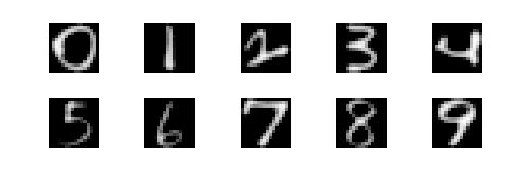
\includegraphics[height=80px]{img/intro_digit_recognition.png}\end{center}
    \begin{itemize}
        \item 1990 год. US Post решили научиться распознавать индексы на конвертах, чтобы автоматически сортировать письма по месту назначения.
        \item Собрали примерно 10К чёрно-белых изображений рукописных цифр 16x16 пикселей. Создали алгоритм, который распознаёт эти цифры.
    \end{itemize}
\end{frame}

\begin{frame}{Примеры. Предсказание оттока пользователей.}
\begin{center}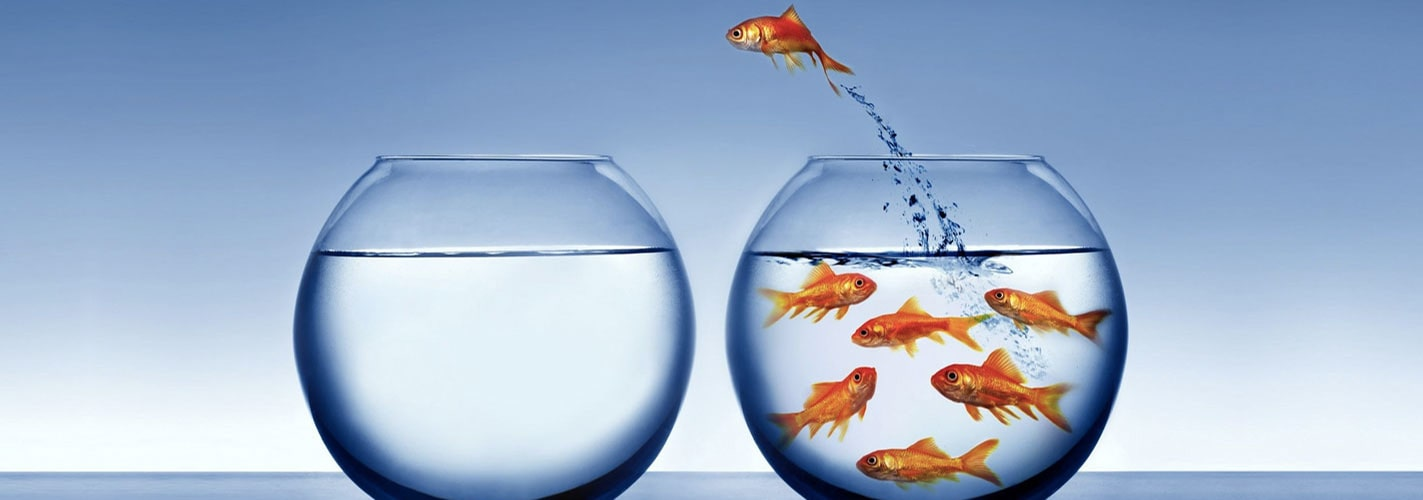
\includegraphics[height=80px]{img/intro_user_churn.jpg}\end{center}
    \begin{itemize}
        \item Изначально проблема пришла из телекома. Во многих видах бизнеса компании выгоднее удерживать старого клиента, чем привлекать нового. Для этого нужно понимать, в какой момент клиент собирается уйти, и в этот момент предложить ему скидку, бесплатный товар, программу лояльности и т.д.
        \item Бинарный классификатор.
        \item Основная проблема в том, что данные динамически меняются: многие свойства клиента меняются по мере его пользования продуктом (например, активность). Нужно выравнивать всех пользователей в разные моменты времени относительно их жизненных циклов.
    \end{itemize}
\end{frame}

\begin{frame}{Примеры. Веб-поиск.}
\begin{tabular}{>{\centering\arraybackslash}m{0.45\textwidth}>{\centering\arraybackslash}m{0.4\textwidth}}
     
\includegraphics[height=20px]{img/intro_yandex.png}
     &\vspace{10px}
\includegraphics[height=25px]{img/intro_google.png}
\end{tabular}

\begin{itemize}
    \item 1997 основан Яндекс. 1998 год основан Google. До этого были другие поисковики (Altavista, Rambler), но они оказались побеждены в том числе по причине невложений в ML.
    \item Поисковый движок решает задачу ранжирования. Важно расставить документы по пользовательскому запросу в порядке их релевантности. То есть не обязательно предсказывать саму релевантность документа. Важно расставить документы в правильном порядке.
    \item В своё время задача стала квинтессенцией современного на тот момент ML. Подобно космонавтике в 1960х.
    \item Развитие поисковых систем совпало с развитием интернета: без них он быстро превращается в помойку. Имея огромное количество пользователей, Google и Яндекс смогли позволить внедрить монетизацию через объявления по очень лояльным для продавца условиям (платишь только за покупку, а не за клик).
    \item Получив большие прибыли, компании продолжили вкладываться в другие технологичные проекты и стали IT-гигантами.
\end{itemize}
\end{frame}

\begin{frame}{Примеры. Рекомендательные системы.}
\begin{center}
\includegraphics[height=50px]{img/intro_netflix.jpg}\end{center}
\begin{itemize}
    \item 2006 год. Netflix \href{https://ru.wikipedia.org/wiki/Netflix_Prize}{проводит соревнование} на построенние лучшей рекомендательной системы на их данных. Приз -- \$1M. Требование: улучшить метрику бейзлайн-алгоритма на 10\%.
    \item Датасет был на 100М оценок, 480К клиентов и 18К фильмов. Предсказывали оценку клиента фильму по шкале 1-5.
    \item Итоги подводили в 2009 году. Две лидирующих команды прислали свои решения с разницей в 20 минут. На открытой тестовой части датасета впереди была одна команда (+10.1\% против +10.09\%), но на закрытой обе показали результат +10.06\%, и победителя определили по времени.
    \item Вложения Netflix в ML стали одним из ключевых пунктов, способствовавших превращению компании из обычного продавца DVD-дисков в гиганта киноиндустрии.
\end{itemize}
\end{frame}

\begin{frame}{Примеры. Распознавание и синтез речи.}
\begin{tabular}{m{0.4\textwidth}m{0.5\textwidth}}
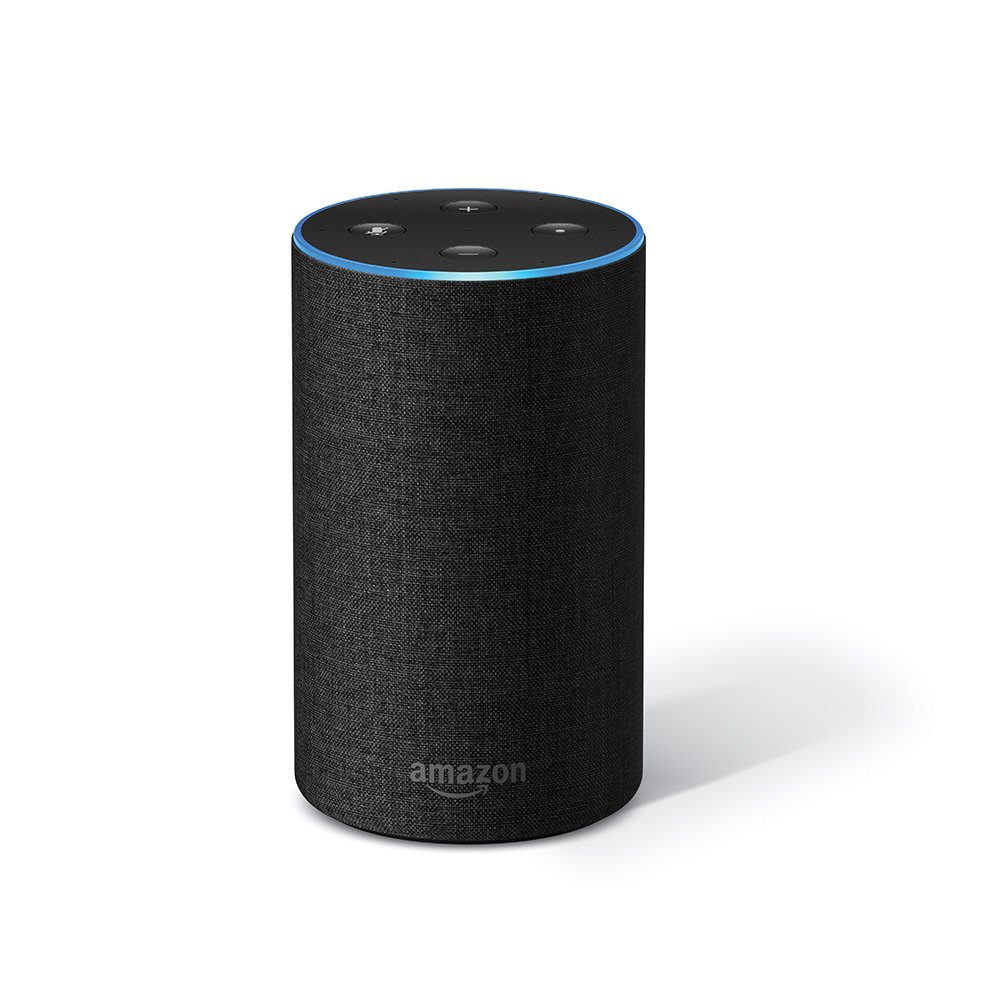
\includegraphics[width=100px]{img/intro_amazon_echo.jpg} & 
\begin{itemize}
    \item Стало возможно после получения прорывных возможностей нейронных сетей в середине 2010х.
    \item Распознавать и синтезировать голос стало намного проще.
    \item Голосовые интерфейсы оказались очень востребованы (например, при управлении автомобилем).
    \item Тренд задал Amazon в 2015, \href{https://ru.wikipedia.org/wiki/Amazon_Echo}{выпустив умную колонку Алекса}. Ещё один пример удачного вложения в ML. Изначально Amazon книгами торговал.
\end{itemize}
\end{tabular}
\end{frame}

\begin{frame}{Примеры. Беспилотные автомобили.}
\begin{center}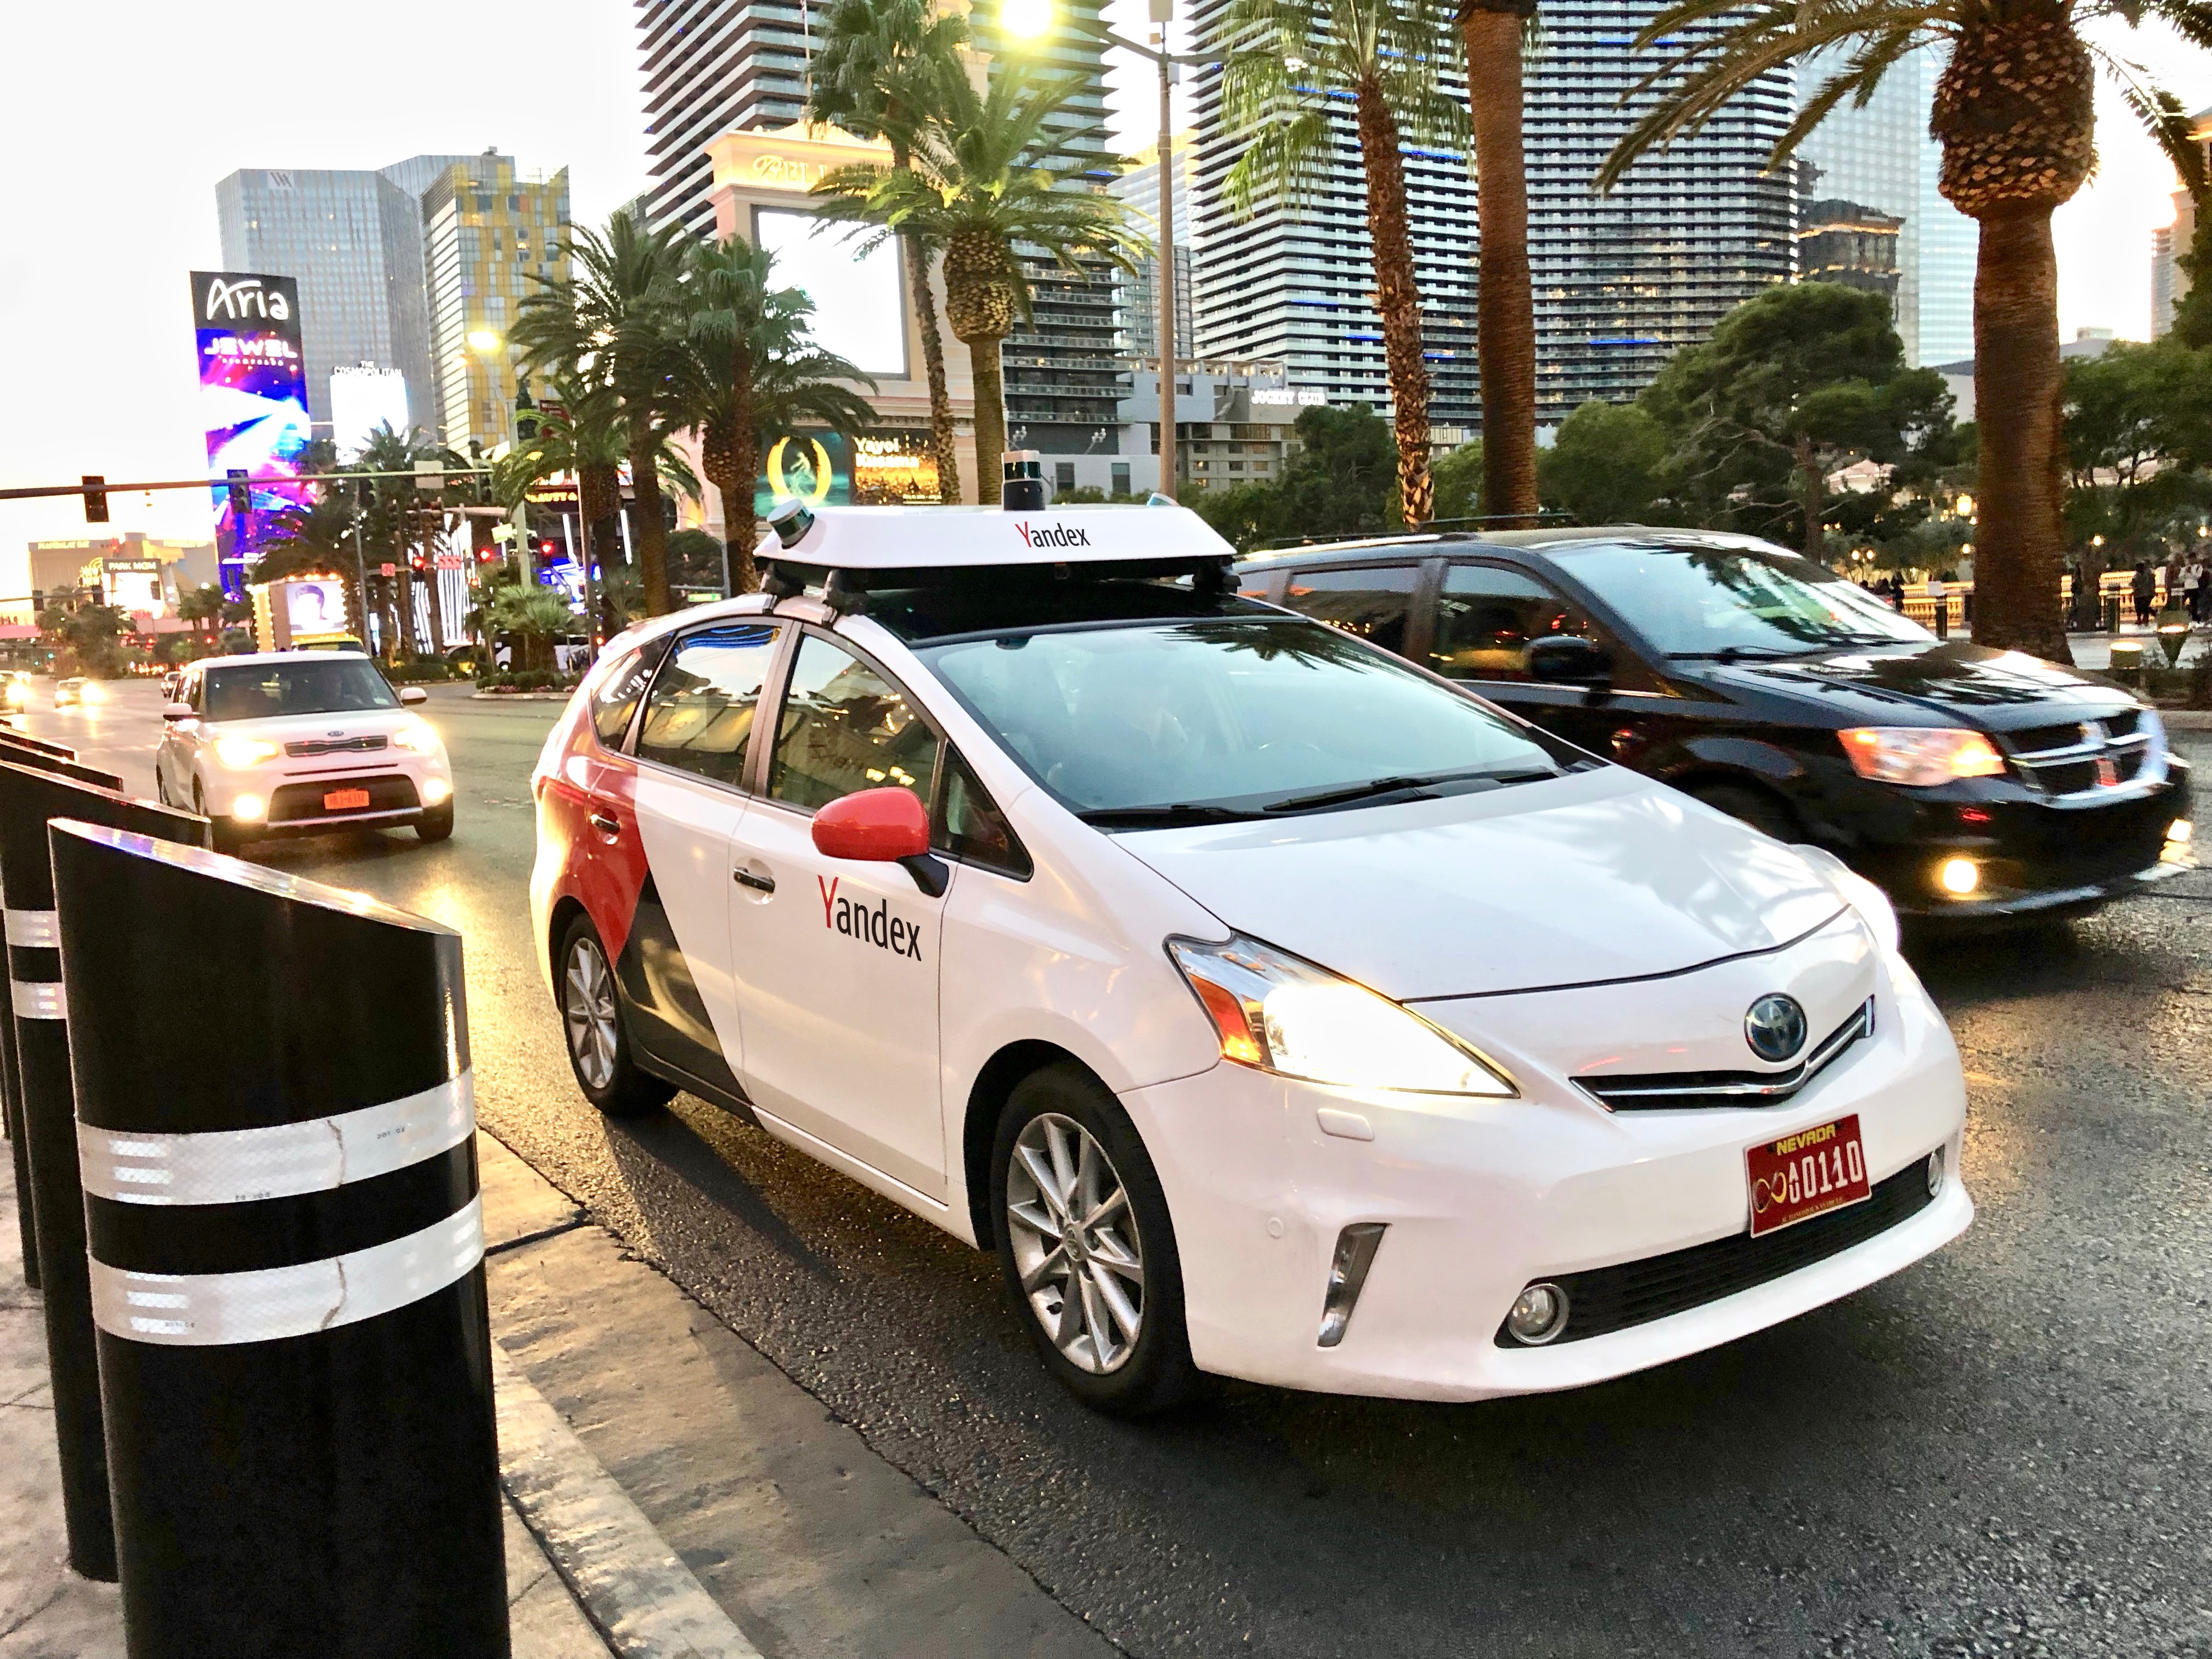
\includegraphics[height=100px]{img/intro_self_driving_cars.jpg}\end{center}
Квинтэссенция ML 2010х. Сочетает в себе огромное количество разных небольших ML-задач:
\begin{itemize}
    \item Управление автомобилем (распознавание образов, анализ дорожной ситуации, оценка рисков, предсказание перемещения объектов)
    \item Навигация. По какому маршруту поехать, чтобы приехать быстрее.
    \item Распознавание голоса, синтез речи.
    \item Прайсинг (пока только для такси): как менять тариф в зависимости от спроса, маршрута и трафика.
    \item Инфраструктура. Нужно быстро обрабатывать огромное количество данных, хранить передавать.
\end{itemize}
\end{frame}


\subsection{Unsupervised learning}
\begin{frame}{Unsupervised learning}
Unsupervised learning -- обучение без учителя -- когда $Y=\varnothing$. То есть нам не нужно подгоняться под таргетную переменную, а нужно, имея данные $X$ сказать что-то про структуру этих данных. Особенность этого типа задач в неоднозначности выбора функционала качества $L$, и в неоднозначости определения оптимальной модели.

Примеры:
\begin{itemize}
    \item Кластерный анализ. Понять, на какие смысловые группы бьются данные.
    \item Поиск аномалий в данных (a.k.a. поиск выбросов, аутлаеров). Аутлаеры -- это нетипичные точки точки в данных, сильно отличающиеся по характеристикам от типичных. Цель задачи: очистить данные.
    \item Поиск ассоциативных правил. Вместе с товаром X также покупают товар Y.
    \item Задачи генерации контента (текста, изображений). На вход подаём множество текстов/фотографий, на выходе хотим получать новые объекты, похожие на объекты из множества обучения.
\end{itemize}
\end{frame}

\end{document}